\section{One-Dimensional Systems}
\noindent\rule[\linienAbstand]{\linewidth}{\linienDickeDick}

\subsection{Fixed points in Continuous Dynamical Systems}
\noindent\rule[\linienAbstand]{\linewidth}{\linienDicke}
A \emph{fixed point} of the a continuous dynamical system is an $x^*$ with the property
\begin{equation}
  \dot{x} = f(x^*) = 0
\end{equation}
If $x^*$ is a fixed point, then $x(t) = x^*$ is a constant solution of the system.\\

For the solution $x(t)$ of a one-dimensional system there are the following possibilites:
\begin{itemize}
  \item The solution is a fixed point
  \item The solution grows monotonically, i.e. $\dot{x}(t) > 0$
  \item The solution decays monotonically, i.e. $\dot{x}(t) < 0$
\end{itemize}

Example: We consider the ODE of limited growth
\begin{equation}
  \dot{N} = rN\left(1-\frac{N}{K}\right)
\end{equation}
If $K = 1$, $\dot{N}$ is $0$ if $N = 0$ and $N = 1$ i.e. the fixed points for this equation are $x_1 = 0$ and $x_2 = 1$ (or $x_2 = K$). These fixed points are also visible in the following figure.

\begin{figure}[H]
  \centering
  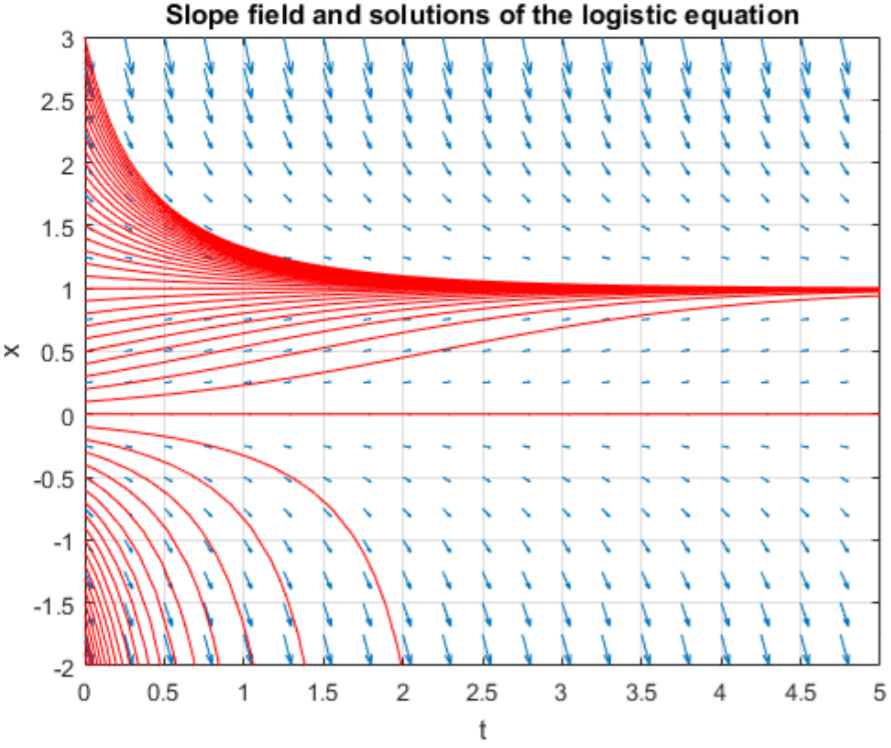
\includegraphics[width=.7\linewidth]{Pics/4.2.png}
\end{figure}

\subsection{Continuous Linear stability analysis}
\noindent\rule[\linienAbstand]{\linewidth}{\linienDicke}
Let $x^*$ be a fixed point of the continuous dynamical system $\dot{x} = f(x)$. The fixed point $x^*$ is
\begin{itemize}
  \item stable if $f'(x^*) < 0$,
  \item unstable, if $f'(x^*) > 0$,
  \item stable or unstable, if $f'(x^*) = 0$
\end{itemize}

Example (continuation): the derivative of the logistic equation above $\left(f(x) = rx\left(1-\frac{x}{K}\right)\right)$ is
\begin{equation}
  f'(x) = r\left(1-\frac{2x}{K}\right)
\end{equation}
Hence
\begin{equation}
  \begin{split}
    f'(x_1) =& f'(0) = r > 0\\
    f'(x_2) =& f'(K) = -r < 0
  \end{split}
\end{equation}
Hence $x_1 = 0$ is an unstable fixed point, and $x_2 = K$ is a stable fixed point, which is also visible in the figure above.

\subsection{Fixed points in Discrete Dynamical Systems}
\noindent\rule[\linienAbstand]{\linewidth}{\linienDicke}
A \emph{fixed point} of the discrete dynamical system $x_{n+1} = f(x_n)$ is a $x^*$ with the property
\begin{equation}
  x^* = f(x^*)
\end{equation}
If $x^*$ is a fixed point of $x_{n+1} = f(x_n)$, then $x_n = x^*$ is a constant solution of that system.\\

Example: We want to find the fixpoint of the discrete dynamical system
\begin{equation}
  x_{n+1} = \textup{cos}(x_n)
\end{equation}
Using the formula above:
\begin{equation}
  x^* = \textup{cos}(x^*) \:\;\; \Rightarrow \;\;\; x^* \approx 0.739
\end{equation}

\subsection{Discrete Linear stability analysis}
\noindent\rule[\linienAbstand]{\linewidth}{\linienDicke}
Let $x^*$ be a fixed point of the discrete dynamical system $x_{n+1} = f(x_n)$. The fixed point $x^*$ is
\begin{itemize}
  \item stable, if $|f'(x^*)| < 1$,
  \item unstable, if $|f'(x^*)| > 1$,
  \item stable or unstable, if  $|f'(x^*)| = 1$
\end{itemize}

\begin{equation}
  \eta_{n+1} = \eta_n \cdot f'(x^*) \;\;\; \Rightarrow \;\;\;
  \eta_n = \eta_0 \cdot \left(f'(x^*)\right)^n
\end{equation}

Example: (continuation): We want to analyse the fixpoint $x^* \approx 0.739$ of the example above.
\begin{equation}
  |f'(x^*)| = |\textup{sin}(x^*)| \approx |-0.674| < 1
\end{equation}
Hence $x^*$ is a stable fixed point of the system.
